\chapter{Ejercicios de clase}
\noindent
Esta sección tiene el propósito de recoger todos los ejercicios propuestos en clase por parte de la profesora y que fueron resueltos por los alumnos en pizarra.

\section{Estadísticos muestrales}
\begin{ejercicio}
    Obtener la función masa de probabilidad conjunta de una m.a.s. de $X\rightsquigarrow B(k_0,p)$ y la función de densidad de una m.a.s. de $X\rightsquigarrow U(a,b)$.\\

    \noindent
    Recordamos que si $X\rightsquigarrow B(k_0, p)$, entonces:
    \begin{equation*}
        P[X = x] = \binom{k_0}{x} p^x{(1-p)}^{n-x} \qquad \forall x\in \{0,\ldots,k_0\}
    \end{equation*}
    Por lo que si tenemos una m.a.s. de $n$ variables independientes e idénticamente distribuidas a $X$, $(X_1, \ldots, X_n)$, su función de densidad vendrá dada por:
    \begin{align*}
        P[X_1 &= x_1, \ldots, X_n = x_n] \stackrel{\text{indep.}}{=} \prod_{i=1}^{n}P[X_i = x_i]\stackrel{\text{id. d.}}{=} \prod_{i=1}^{n} P[X=x_i] \\
              &= \prod_{i=1}^{n} \binom{k_0}{x_i} p^{x_i} {(1-p)}^{k_0-x_i} = p^{\sum\limits_{i=1}^{n}x_i} {(1-p)}^{nk_0 - \sum\limits_{i=1}^{n}x_i} \prod_{i=1}^{n}\binom{k_0}{x_i} \\
              & \qquad \forall x_i \in \{0,\ldots,k_0\}
    \end{align*}

    \noindent
    Si ahora $X\rightsquigarrow U(a,b)$ para ciertos $a,b\in \mathbb{R}$ con $a<b$, entonces:
    \begin{equation*}
        f_X(x) = \dfrac{1}{b-a} \qquad \forall x\in [a,b]
    \end{equation*}

    de donde:
    \begin{equation*}
        f_{(X_1, \ldots, X_n)}(x_1, \ldots, x_n) \stackrel{\text{indep.}}{=} \prod_{i=1}^{n} f_{X_i}(x_i)\stackrel{\text{id. d.}}{=} \prod_{i=1}^{n} f_X(x_i) = \prod_{i=1}^{n} \dfrac{1}{b-a} = \dfrac{1}{{(b-a)}^{n}} \qquad \forall x\in [a,b]
    \end{equation*}
\end{ejercicio}

\begin{ejercicio}
    Para cada realización muestral, $(x_1, \ldots, x_n)\in \cc{X}^n$, $F_{x_1,\ldots,x_n}^\ast$ es una función de distribución en $\mathbb{R}$. En particular es una función a saltos, con saltos de amplitud $\nicefrac{1}{n}$ en los sucesivos valores muestrales ordenados de menor a mayor, supuestos que sean distintos, y de saltos múltiplos en el caso de que varios valores muestrales coincidieran.\\

    \noindent
    En las condiciones del enunciado, es decir, suponiendo que $x_1, \ldots, x_n$ están ordenados de menor a mayor y son distintos, entonces es fácil ver que:
    \begin{equation*}
        F_{x_1, \ldots, x_n}^\ast (x) = \left\{\begin{array}{ll}
                0 & \text{si\ } x < x_1 \\
                \nicefrac{1}{n} & \text{si\ } x_1 \leq x < x_2 \\
                                &\vdots \\
                            1 & \text{si\ } x > x_n
        \end{array}\right. \qquad \forall x\in \mathbb{R}
    \end{equation*}
    Por lo que es claro que $F_{x_1, \ldots, x_n}^\ast $ es no decreciente, continua por la derecha, con límite 0 en $-\infty$ y con límite 1 en $+\infty$.
\end{ejercicio}

\begin{ejercicio}
    Para todo $x\in \mathbb{R}$, $F_{X_1, \ldots, X_n}^\ast(x)$ es una variable aleatoria tal que \newline $nF_{X_1, \ldots, X_n}^\ast(x) \rightsquigarrow B(n,F(x))$ y:
    \begin{equation*}
        E[F_{X_1, \ldots, X_n}^\ast (x)] = F(x), \qquad Var[F_{X_1, \ldots, X_n}^\ast (x)] = \dfrac{F(x)(1-F(x))}{n}
    \end{equation*}
    donde $F(x)$ es la función de distribución de $X$.\\

    \noindent
    Recordamos que:
    \begin{equation*}
    F_{X_1, \ldots, X_n}^\ast (x) = \dfrac{1}{n}\sum_{i=1}^{n}I_{\left]-\infty,x\right]}(X_i) \qquad \forall x\in \mathbb{R}
    \end{equation*}
Fijado $x\in \mathbb{R}$, tenemos que $I_{\left]-\infty,x\right]}(X)\rightsquigarrow B(1,P[X\leq x]) \equiv B(1,F(x))$, por lo que por la propiedad reproductiva de la binomial tenemos que:
    \begin{equation*}
        nF_{X_1, \ldots, X_n}^\ast (x) \rightsquigarrow B(n,F(x))
    \end{equation*}
    Por lo que:
    \begin{equation*}
        nE[F_{X_1, \ldots, X_n}^\ast (x)] = E[nF_{X_1, \ldots, X_n}^\ast (x)] = nF(x)
        \Longrightarrow
        E[F_{X_1, \ldots, X_n}^\ast (x)] = F(x)
    \end{equation*}
    Para la varianza:
    \begin{multline*}
        n^2Var[F_{X_1, \ldots, X_n}^\ast (x)] = Var[nF_{X_1, \ldots, X_n}^\ast (x)] = nF(x)(1-F(x))
        \Longrightarrow \\ \Longrightarrow
        Var[F_{X_1, \ldots, X_n}^\ast (x)] = \dfrac{F(x)(1-F(x))}{n}
    \end{multline*}
\end{ejercicio}

\begin{ejercicio}
    Para valores grandes de $n$, en virtual del Teorema Central del Límite:
    \begin{equation*}
        F_{X_1, \ldots, X_n}^\ast (x) \rightsquigarrow \cc{N}\left(F(x), \dfrac{F(x)(1-F(x))}{n}\right)
    \end{equation*}

    \noindent
    Sea $(X_1, \ldots, X_n)$ una m.a.s. de $n$ muestras, sea:
    \begin{equation*}
        S_n = \sum_{i=1}^{n} I_{\left]-\infty,x\right]}(X_i) \qquad \forall n\in \mathbb{N}
    \end{equation*}
    Por el Teorema Central del Límite tenemos que:
    \begin{equation*}
        \dfrac{S_n - E[S_n]}{\sqrt{Var[S_n]}} \stackrel{n\to \infty}{\rightsquigarrow} \cc{N}(0,1) \Longrightarrow S_n \stackrel{n\to \infty}{\rightsquigarrow} \cc{N}\left(E[S_n], Var[S_n]\right)
    \end{equation*}
    Como $S_n \rightsquigarrow B(n,F(x))$, entonces tenemos que:
    \begin{align*}
        E[S_n] &= nF(x) \\
        Var[S_n] &= nF(x)(1-F(x))
    \end{align*}
    Por lo que:
    \begin{equation*}
        F_{X_1, \ldots, X_n}^\ast (x) = \dfrac{1}{n}S_n \stackrel{n\to \infty}{\rightsquigarrow} \cc{N}\left(F(x), \dfrac{F(x)(1-F(x))}{n}\right)
    \end{equation*}
\end{ejercicio}

\begin{ejercicio}
    Dada una muestra aleatoria simple formada por las observaciones $(3, 8, 5, 4, 5)$, obtener su función de distribución muestral y realizar la representación gráfica.\\

    \noindent
    Aplicando la definición de la función de distribución muestral obtenemos que:
    \begin{equation*}
        F_{(3, 8, 5, 4, 5)}^\ast(x) = \left\{\begin{array}{ll}
                0 & \text{si\ } x < 3 \\
                \nicefrac{1}{5} & \text{si\ } 3 \leq x < 4 \\
                \nicefrac{2}{5} & \text{si\ } 4 \leq x < 5 \\
                \nicefrac{4}{5} & \text{si\ } 5 \leq x < 8 \\
                1 & \text{si\ } x \geq 8 
        \end{array}\right.
    \end{equation*}

    \begin{figure}[H]
        \centering
        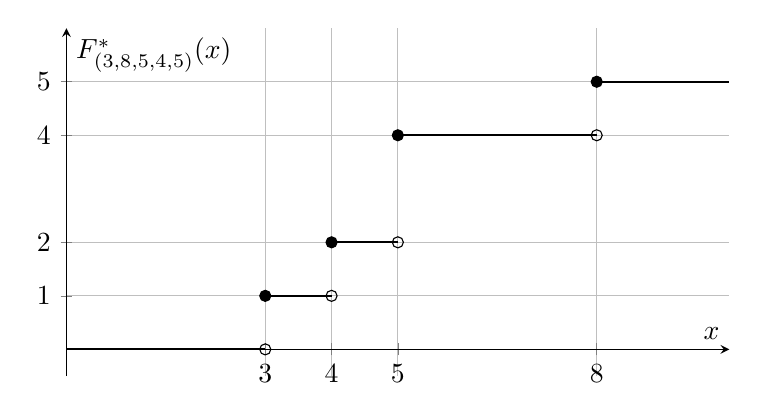
\begin{tikzpicture}
        \begin{axis}[
            axis lines=middle,
            xlabel={$x$},
            ylabel={$F_{(3,8,5,4,5)}^\ast (x)$},
            ymin=-0.5, ymax=6,
            xmin=0, xmax=10,
            xtick={3,4,5,8},
            ytick={0,1,2,4,5},
            grid=both,
            width=10cm,
            height=6cm
        ]

        % Tramos de la función
        \addplot[domain=0:3, thick] {0};

        \addplot[domain=3:4, thick] {1};
        \addplot[domain=4:5, thick] {2};
        \addplot[domain=5:8, thick] {4};
        \addplot[domain=8:10, thick] {5};

        % Puntos abiertos y cerrados
        \addplot[only marks, mark=o] coordinates {(3,0) (4,1) (5,2) (8,4)};
        \addplot[only marks, mark=*] coordinates {(3,1) (4,2) (5,4) (8,5)};

        \end{axis}
        \end{tikzpicture}
        \caption{Representación gráfica de $F_{(3,8,5,4,5)}^\ast (x)$.}
    \end{figure}
\end{ejercicio}

\begin{ejercicio}
    Sea $X$ una variable aleatoria con distribución $B(1,p)$ con $p\in (0,1)$. Se toma una muestra de tamaño 5, $(X_1, X_2, X_3, X_4, X_5)$, y se obtiene la siguiente observación $(0,1,1,0,0)$. Determinar el valor de los estadísticos estudiados en la observación.\\

    \noindent
    Aplicando las fórmulas vistas en clase obtenemos:
    \begin{itemize}
        \item Media:
        \begin{equation*}
            \overline{X} = \dfrac{0+1+1+0+0}{5} = 0.4
        \end{equation*}
        \item Varianza muestral:
        \begin{equation*}
            \sigma^2 = \dfrac{(0-0.4)^2 + (1-0.4)^2 + (1-0.4)^2 + (0-0.4)^2 + (0-0.4)^2}{5} = \dfrac{1.2}{5} = 0.24
        \end{equation*}
        \item Cuasivarianza:
        \begin{equation*}
            s^2 = \dfrac{(0-0.4)^2 + (1-0.4)^2 + (1-0.4)^2 + (0-0.4)^2 + (0-0.4)^2}{5-1} =
            \dfrac{1.2}{4} = 0.3
        \end{equation*}
        \item Estadísticos ordenados:
        \begin{equation*}
            x_{(1)} = 0, \quad x_{(2)} = 0, \quad x_{(3)} = 0, \quad x_{(4)} = 1, \quad x_{(5)} = 1
        \end{equation*}
    \end{itemize}
\end{ejercicio}

\begin{ejercicio}
    Sea $(X_1, \ldots, X_n)$ una m.a.s. y $\overline{X} = \dfrac{1}{n}\sum\limits_{i=1}^{n}X_i$, entonces:
    \begin{equation*}
        M_{\overline{X}}(t) = {(M_X(\nicefrac{t}{n}))}^{n}
    \end{equation*}
    \begin{equation*}
        M_{\overline{X}}(t) = E\left[e^{t\overline{X}}\right] = E\left[e^{\frac{t}{n}\sum\limits_{i=1}^{n}X_i}\right] = M_{\sum\limits_{i=1}^{n}X_i}\left(\frac{t}{n}\right) \stackrel{\text{indep.}}{=} \prod_{i=1}^{n} M_{X_i}\left(\frac{t}{n}\right) \stackrel{\text{id. d.}}{=} {\left(M_X\left(\frac{t}{n}\right)\right)}^{n}
    \end{equation*}
\end{ejercicio}

\begin{ejercicio}\label{ej:dist_muestral_media}
    Obtener la distribución muestral de $\overline{X}$ para $(X_1, \ldots, X_n)$ una m.a.s. de $X\rightsquigarrow \cc{N}(\mu, \sigma^2)$.

    \begin{equation*}
        M_{\overline{X}}(t) = {\left(M_X\left(\frac{t}{n}\right)\right)}^{n} = {\left(e^{\frac{\mu t}{n} + \frac{\sigma^2 t^2}{2n^2}}\right)}^{n} = e^{\mu t + \frac{\sigma^2 t^2}{2n}}
    \end{equation*}
    Luego $\overline{X}\rightsquigarrow \cc{N}\left(\mu, \frac{\sigma^2}{n}\right)$, ya que la función generatriz de momentos caracteriza la distribución.
\end{ejercicio}

\begin{prop}
    Si tenemos una m.a.s. $(X_1, \ldots, X_n)$, entonces:
    \begin{align*}
        F_{X_{(n)}}(x) &= {(F_X(x))}^{n} \qquad \forall x\in \mathbb{R} \\
        F_{X_{(1)}}(x) &= 1-{(1-F_X(x))}^{n}
    \end{align*}
    \begin{proof}
        Para la distribución del máximo:
        \begin{align*}
            F_{X_{(n)}}(x) &= P[X_{(n)} \leq x] = P[X_1 \leq x, \ldots, X_n \leq x] \stackrel{\text{indep.}}{=} \prod_{i=1}^{n} P[X_i \leq x] \\ &\stackrel{\text{id. d.}}{=} \prod_{i=1}^{n} P[X\leq x] = {(F_X(x))}^{n}
        \end{align*}
        Para la del mínimo:
        \begin{align*}
            F_{X_{(1)}}(x) &= P[X_{(1)}\leq x] = 1-P[X_{(1)} > x] = 1-P[X_1 > x, \ldots, X_n > x] \\ &\stackrel{\text{indep.}}{=} 1 - \prod_{i=1}^{n}P[X_i > x] \stackrel{\text{id. d.}}{=} 1-{(P[X>x])}^{n} = 1-{(1-F_X(x))}^{n}
        \end{align*}
    \end{proof}
\end{prop}

\begin{ejercicio}
    Obtener las distribuciones muestrales de $X_{(1)}$ y  $X_{(n)}$ para \newline $X\rightsquigarrow U(a,b)$.\\

    \noindent
    Si $X\rightsquigarrow U(a,b)$, entonces:
    \begin{equation*}
        F_X(x) = \dfrac{x-a}{b-a} \qquad \forall x\in [a,b]
    \end{equation*}
    Por lo que aplicando la Proposición superior:
    \begin{align*}
        F_{X_{(n)}}(x) &= {(F_X(x))}^{n} = {\left(\dfrac{x-a}{b-a}\right)}^{n} \qquad \forall x\in [a,b] \\
        F_{X_{(1)}}(x) &= 1 - {(1-F_X(x))}^{n} = 1-{\left(1-\dfrac{x-a}{b-a}\right)}^{n} 
        = 1-{\left(\dfrac{b-x}{b-a}\right)}^{n} \qquad \forall x\in [a,b]
    \end{align*}
\end{ejercicio}

\begin{ejercicio}
    Sea $(X_1, \ldots, X_n)$ una m.a.s. de $X$. Entonces, para los momentos no centrados de orden $k$ de la m.a.s. se tiene que:
    \begin{align*}
        E\left[A_k\right] &= E[X^k] \\
        Var\left[A_k\right] &= \dfrac{Var[X^k]}{n}
    \end{align*}

    Demostremos la primera igualdad:
    \begin{align*}
        E\left[A_k\right] &= E\left[\dfrac{1}{n}\sum_{i=1}^{n}X_i^k\right] = \dfrac{1}{n}\sum_{i=1}^{n}E[X_i^k]
        \stackrel{\text{id. d.}}{=} \dfrac{1}{n}\sum_{i=1}^{n}E[X^k] = E[X^k]
    \end{align*}

    Demostremos la segunda igualdad:
    \begin{align*}
        Var\left[A_k\right] &= Var\left[\dfrac{1}{n}\sum_{i=1}^{n}X_i^k\right] = \dfrac{1}{n^2}Var\left[\sum_{i=1}^{n}X_i^k\right]
        \stackrel{\text{indep.}}{=} \dfrac{1}{n^2}\sum_{i=1}^{n}Var[X_i^k]
        \stackrel{\text{id. d.}}{=}\\&\stackrel{\text{id. d.}}{=}
        \dfrac{1}{n^2}\sum_{i=1}^{n}Var[X^k] = \dfrac{Var[X^k]}{n}
    \end{align*}
\end{ejercicio}

\section{Distribuciones en el muestreo de poblaciones normales}
\begin{prop}
    Sea $X\rightsquigarrow\cc{N}(0,1)$, entonces $X^2\rightsquigarrow \chi^2(1)$.
    \begin{proof}
        Sea $Y = X^2 = h(X)$, entonces $X = \pm \sqrt{Y} = h^{-1}(y)$, por lo que:
        \begin{equation*}
            f_Y(y) = f_X(h_1^{-1}(y)) \left|\dfrac{dh_1^{-1}(y)}{dy}\right| + f_X(h_2^{-1}(y)) + \left|\dfrac{dh_2^{-1}(y)}{dy}\right| 
        \end{equation*}
        Como $X\rightsquigarrow \cc{N}(0,1)$, entonces:
        \begin{equation*}
            f_X(x) = \dfrac{1}{\sqrt{2\pi}} e^{\frac{-x^2}{2}} \qquad \forall x\in \mathbb{R}
        \end{equation*}
        De donde:
        \begin{equation*}
            f_Y(y) = \dfrac{1}{\sqrt{2\pi}} e^{\frac{-{(\sqrt{y})}^{2}}{2}} \left|\dfrac{1}{2\sqrt{y}}\right| + \dfrac{1}{\sqrt{2\pi}} e^{\frac{-{(-\sqrt{y})}^{2}}{2}} \left|\dfrac{-1}{2\sqrt{y}}\right|  = \dfrac{1}{\sqrt{2\pi y}} e^{\frac{-y}{2}} \qquad \forall y>0
        \end{equation*}
        Por lo que $Y\rightsquigarrow\chi^2(1)$.
    \end{proof}
\end{prop}

\begin{ejercicio}
    Calcula el valor de $k$ o la probabilidad inducida:
    \begin{enumerate}[label=\alph*)]
        \item $P[\chi^2(10)\geq k] = 0.005$.

            Consultando la tabla de la distribución $\chi^2$, obtenemos que $k = 25.1881$.
        \item $P[\chi^2(45) \leq k] = 0.005$.
        
            Tenemos que:
            \begin{equation*}
                P[\chi^2(45) \leq k] = 1-P[\chi^2(45) \geq k] = 0.005 \Longrightarrow
                P[\chi^2(45) \geq k] = 0.995
            \end{equation*}
            Consultando la tabla de la distribución $\chi^2$, obtenemos que $k = 24.3110$.
        
        \item $P[\chi^2(14) \geq 21.06]$
        
            En este caso, no podemos consultar de forma directa los encabezados de la tabla de la distribución $\chi^2$ y obtener el valor de la probabilidad, sino que tenemos que buscar qué columna de la tabla contiene el valor buscado. Podemos ver que:
            \begin{equation*}
                P[\chi^2(14) \geq 21.06] \approx 0.1
            \end{equation*}
            
        \item $P[\chi^2(20) \leq 12.44]$
        
            Tenemos que:
            \begin{equation*}
                P[\chi^2(20) \leq 12.44] = 1-P[\chi^2(20) \geq 12.44] \AstIg 1-0.9 = 0.1
            \end{equation*}
            donde en $(\ast)$ hemos consultado la tabla de la distribución $\chi^2$.
    \end{enumerate}
\end{ejercicio}

\begin{ejercicio}
    Calcula el valor de $k$ o la probabilidad inducida:
    \begin{enumerate}[label=\alph*)]
        \item $P[t(26)\geq k] = 0.05$

            Consultando la tabla de la distribución $t$ de Student, obtenemos que $k = 1.706$.
        \item $P[t(20)\leq k] = 0.25$
        
            Por la simetría de la distribución $t$ de Student, tenemos que:
            \begin{equation*}
                0.25 = P[t(20)\leq k] = P[t(20)\geq -k]
            \end{equation*}

            Consultando la tabla de la distribución $t$ de Student, obtenemos que $-k = 0.6870$, luego $k = -0.6870$.
        \item $P[t(26) \geq k] = 0.9$

            Tenemos que:
            \begin{equation*}
                0.9 = P[t(26) \geq k] = 1-P[t(26) \leq k] = 1-P[t(26) \geq -k] \Longrightarrow P[t(26) \geq -k] = 0.1
            \end{equation*}

            Consultando la tabla de la distribución $t$ de Student, obtenemos que $-k = 1.3150$, luego $k = -1.3150$.
        \item $P[t(21) \geq 1.721]$

            Consultando la tabla de la distribución $t$ de Student, obtenemos que:
            \begin{equation*}
                P[t(21) \geq 1.721] \approx 0.05
            \end{equation*}
        \item $P[t(11) \leq 0.697]$
        
            Consultando la tabla de la distribución $t$ de Student, obtenemos que:
            \begin{equation*}
                P[t(11) \leq 0.697] = 1-P[t(11) \geq 0.697] \approx 1-0.25 = 0.75
            \end{equation*}
        \item $P[t(8) \leq -2.306]$
        
            Tenemos que:
            \begin{equation*}
                P[t(8) \leq -2.306] = P[t(8) \geq 2.306] = 0.025
            \end{equation*}
    \end{enumerate}
\end{ejercicio}

\begin{ejercicio}
    Calcula el valor de $k$ o la probabilidad inducida:
    \begin{enumerate}[label=\alph*)]
        \item $P[F(7,3) \leq k] = 0.95$
        
            Consultando de manera directa la tabla de la distribución $F$ de Snedecor, obtenemos que $k = 8.89$.
        \item $P[F(8,4) \geq k] = 0.01$
            \begin{equation*}
                0.01 = P[F(8,4) \geq k] = 1 - P[F(8,4) \leq k] \Longrightarrow P[F(8,4) \leq k] = 0.99
            \end{equation*}
            Consultando la tabla de la distribución $F$ de Snedecor, obtenemos que $k = 14.8$.
        \item $P[F(2,2) \leq 19]$
        
            Consultando la tabla de la distribución $F$ de Snedecor, obtenemos que:
            \begin{equation*}
                P[F(2,2) \leq 19] = 0.95
            \end{equation*}
        \item $P[F(3,5) \geq 12.1]$
            \begin{equation*}
                P[F(3,5) \geq 12.1] = 1-P[F(3,5) \leq 12.1] \AstIg 1-0.99 = 0.01
            \end{equation*}
            donde en $(\ast)$ hemos consultado la tabla de la distribución $F$ de Snedecor.
        \item $P[F(60,40) \leq k] = 0.05$
            
            Consultando la tabla de la distribución $F$ de Snedecor, obtenemos que $k = 0.627$.
    \end{enumerate}
\end{ejercicio}

\subsection{Muestreo en una población normal unidimensional}
En lo que sigue, sea una $(X_1, \ldots, X_n)$ m.a.s. con $X\rightsquigarrow \cc{N}(\mu, \sigma^2)$.

\begin{prop}
    En dichas condiciones, veamos que:
    \begin{equation*}
        \overline{X}, (X_1 - \overline{X}, \ldots, X_n - \overline{X}) \text{\ son independientes}
    \end{equation*}
    \begin{proof}
        Para ellos, usaremos la caracterización de independencia de vectores aleatorios por la función generatriz de momentos conjunta. Es decir, buscamos probar
        \begin{equation*}
            M_{\overline{X},X_1 - \overline{X}, \ldots, X_n - \overline{X}}(t,t_1, \ldots, t_n) \stackrel{\text{?}}{=} M_{\overline{X}}(t) M_{X_1 - \overline{X}, \ldots, X_n - \overline{X}}(t_1, \ldots, t_n)
        \end{equation*}

        Por la reproductividad de la normal, todas las variables aleatorias que aparecen son normales, luego su función característica de momentos está definida en todo $\bb{R}$. Por tanto, para todo $(t, t_1, \ldots, t_n)\in \bb{R}^{n+1}$, tenemos que:
        \begin{align*}
            M_{\overline{X},X_1 - \overline{X}, \ldots, X_n - \overline{X}}&(t, t_1, \ldots, t_n) 
            = E\left[e^{(t, t_1, \ldots, t_n) \cdot (\overline{X},X_1 - \overline{X}, \ldots, X_n - \overline{X})}\right]
            = E\left[e^{t\overline{X} + \sum\limits_{i=1}^{n}(X_i - \overline{X})t_i}\right] 
            =\\&= E\left[e^{\frac{t}{n}\sum\limits_{i=1}^n X_i + \sum\limits_{i=1}^n X_it_i - \sum\limits_{i=1}^n \overline{X}t_i}\right] 
            = E\left[e^{\frac{t}{n}\sum\limits_{i=1}^n X_i + \sum\limits_{i=1}^n X_it_i - \overline{X}\sum\limits_{i=1}^n t_i}\right] 
            =\\&= E\left[e^{\frac{t}{n}\sum\limits_{i=1}^n X_i + \sum\limits_{i=1}^n X_it_i - \frac{1}{n}\sum\limits_{i=1}^n X_i\sum\limits_{i=1}^n t_i}\right] 
            = E\left[e^{\frac{t}{n}\sum\limits_{i=1}^n X_i + \sum\limits_{i=1}^n X_it_i - \sum\limits_{i=1}^n X_i\frac{1}{n}\sum\limits_{i=1}^n t_i}\right] 
            =\\&= E\left[e^{\frac{t}{n}\sum\limits_{i=1}^n X_i + \sum\limits_{i=1}^n X_it_i - \sum\limits_{i=1}^n X_i\overline{t}}\right] 
            = E\left[e^{\sum\limits_{i=1}^n X_i\frac{t}{n} + \sum\limits_{i=1}^n X_it_i - \sum\limits_{i=1}^n X_i\overline{t}}\right] 
            =\\&= E\left[e^{\sum\limits_{i=1}^n X_i \left(\frac{t}{n} + t_i - \overline{t}\right)}\right] 
            = E\left[\prod_{i=1}^{n}e^{X_i\left(\frac{t}{n}+t_i - \overline{t}\right)}\right] 
            \stackrel{\text{indep.}}{=} \prod_{i=1}^{n} E\left[e^{X_i\left(\frac{t}{n}+t_i - \overline{t}\right)}\right]
            =\\&= \prod_{i=1}^{n} M_{X_i}\left(\frac{t}{n}+t_i - \overline{t}\right) 
            \AstIg \prod_{i=1}^{n} \exp\left[\left(\frac{t}{n}+t_i-\overline{t}\right)\mu + {\left(\frac{t}{n}+t_i - \ol{t}\right)}^{2}\frac{\sigma^2}{2}\right]
            =\\&=\exp\left[\sum\limits_{i=1}^n \left[\left(\frac{t}{n}+t_i - \overline{t}\right)\mu + \frac{\sigma^2}{2} \left(\frac{t^2}{n^2} + {\left(t_i - \overline{t}\right)}^{2} + 2\frac{t}{n}(t_i - \overline{t})\right)\right]\right] 
            =\\&= \exp\left[\sum\limits_{i=1}^n \frac{\mu t}{n} + \sum\limits_{i=1}^n \mu (t_i-\overline{t}) + \frac{\sigma^2}{2}\left(\sum\limits_{i=1}^n \frac{t^2}{n^2} + \sum\limits_{i=1}^n {(t_i - \overline{t})}^{2} + 2\sum\limits_{i=1}^n \frac{t}{n}(t_i - \overline{t}) \right)\right]
            \stackrel{(\ast\ast)}{=}\\&\stackrel{(\ast\ast)}{=} \exp\left[\frac{\cancel{n}\mu t}{\cancel{n}} + \mu \cancel{\sum\limits_{i=1}^n (t_i - \overline{t})} + \frac{\sigma^2}{2} \left(\frac{\cancel{n}t^2}{n^{\cancel{2}}} + \sum\limits_{i=1}^n {(t_i - \overline{t})}^{2} + 2\frac{t}{n}\cancel{\sum\limits_{i=1}^n (t_i - \overline{t})}\right)\right]
            =\\&= \exp\left[\mu t + \frac{\sigma^2t^2}{2n} + \frac{\sigma^2}{2}\sum\limits_{i=1}^n {(t_i - \overline{t})}^2{}\right]
        \end{align*}
        donde en $(\ast)$ hemos usado que todas las variables son idénticamente distribuidas a una $\cc{N}(\mu, \sigma^2)$; y en $(\ast\ast)$ hemos usado que el momento centrado de primer orden es cero.
        Sabemos que:
        \begin{align*}
            M_{\overline{X}}(t) &= M_{\left(\overline{X},X_1 - \overline{X}, \ldots, X_n - \overline{X}\right)}(t,0, ..., 0) = e^{\mu t + \frac{\sigma^2t^2}{2n}} \\
            M_{(X_1 - \overline{X}, \ldots, X_n - \overline{X})}(t_1, ..., t_n) &= M_{(\overline{X},X_1 - \overline{X}, \ldots, X_n - \overline{X})}(0,t_1, \ldots, t_n) \\
                                &= e^{\frac{\sigma^2}{2}\sum\limits_{i=1}^n {(t_i - \overline{t})}^{2}}
        \end{align*}

        Por tanto, tenemos que el producto de las funciones generatrices de momentos es la generatriz de mmoentos conjunta, luego las variables son independientes.
    \end{proof}
\end{prop}

\begin{coro}\label{cor:muestreo_1normal}
    En dichas condiciones, tenemos que:
    \begin{enumerate}
        \item $\ol{X}\rightsquigarrow \cc{N}(\mu, \frac{\sigma^2}{n})$
        \item (Lema de Fisher): $\ol{X}$ y $S^2$ son independientes.
        \item $\dfrac{(n-1)S^2}{\sigma^2}\rightsquigarrow \chi^2(n-1)$
        \item $\dfrac{\ol{X}-\mu}{\nicefrac{S}{\sqrt{n}}}\rightsquigarrow t(n-1)$
    \end{enumerate}
\begin{proof}
    Demostramos cada una de las afirmaciones:
    \begin{itemize}
        \item Se vio ya en el Ejercicio~\ref{ej:dist_muestral_media}.
        \item Como $S^2$ es función del vector de la Proposición anterior, tenemos que es independiente a $\overline{X}$, ya que las funciones de variables independientes son independientes.
        \item Queremos demostrar que:
            \begin{equation*}
                \dfrac{(n-1)S^2}{\sigma^2} = \dfrac{\sum\limits_{i=1}^n {(X_i - \overline{X})}^{2}}{\sigma^2} \rightsquigarrow\chi^2(n-1)
            \end{equation*}
            
            Tenemos que:
            \begin{align*}
                \dfrac{\sum\limits_{i=1}^n {(X_i - \mu)}^{2}}{\sigma^2} &= \dfrac{\sum\limits_{i=1}^n{(X_i - \overline{X} + \overline{X} - \mu)}^{2}}{\sigma^2} \\ 
                &= \dfrac{\sum\limits_{i=1}^n {(X_i - \overline{X})}^{2} + \sum\limits_{i=1}^n {(\overline{X}-\mu)}^{2} + 2\cancel{\sum\limits_{i=1}^n (X_i - \overline{X})}(\overline{X} - \mu)}{\sigma^2} \\
                &= \dfrac{\sum\limits_{i=1}^n {(X_i - \overline{X})}^{2} }{\sigma^2} + n \dfrac{{(\overline{X}-\mu)}^{2}}{\sigma^2}
            \end{align*}

            Notemos que estamos interesados en conocer la distribución de la primera parte de la suma. Notemos por $A$ a la suma completa, por $B$ a la primera parte y por $C$ a la segunda parte, de forma que $A=B+C$.            
            Veamos la distribución de cada término:
            \begin{itemize}
                \item Por un lado para $A$, tenemos que:
                \begin{equation*}
                    A = \dfrac{\sum\limits_{i=1}^n {(X_i - \mu)}^{2}}{\sigma^2} =
                    \sum\limits_{i=1}^n {\left(\dfrac{X_i - \mu}{\sigma}\right)}^{2} \AstIg \sum\limits_{i=1}^n Z_i^2 \rightsquigarrow \chi^2(n)
                \end{equation*}
                donde en $(\ast)$ hemos usado que $X_i\rightsquigarrow \cc{N}(\mu, \sigma^2)$, por lo que su variable tipificada $Z_i\rightsquigarrow \cc{N}(0,1)$. Además, en la última igualdad hemos empleado la construcción de la distribución $\chi^2$ a partir de variables normales.
                \item Por otro lado, para $C$, del Ejercicio~\ref{ej:dist_muestral_media}, tenemos que $\ol{X}\rightsquigarrow \cc{N}(\mu, \frac{\sigma^2}{n})$, por lo que, tipificando 
                \begin{equation*}
                    \dfrac{\ol{X}-\mu}{\sqrt{\nicefrac{\sigma^2}{n}}} = \dfrac{\ol{X}-\mu}{\nicefrac{\sigma}{\sqrt{n}}}=\sqrt{n}\dfrac{\ol{X}-\mu}{\sigma} \rightsquigarrow \cc{N}(0,1)
                \end{equation*}

                Elevando al cuadrado y empleando la construcción de la distribución $\chi^2$, obtenemos que:
                \begin{equation*}
                    C = n\dfrac{{(\ol{X}-\mu)}^{2}}{\sigma^2} \rightsquigarrow \chi^2(1)
                \end{equation*}
            \end{itemize}

            Buscamos la distribución de $B$, y para ello, buscamos su caracterización por la función generatriz de momentos. Tenemos que $B=f(S^2)$, mientras que $C=g(\ol{X})$. Como, por el Lema de Fisher, $\ol{X}$ y $S^2$ son independientes, tenemos que $B$ y $C$ son independientes. Por lo que:
            \begin{equation*}
                M_{A=B+C}(t) \stackrel{\text{indep.}}{=} M_B(t) M_C(t)
            \end{equation*}

            Veamos la función generatriz de momentos de $A$ y $C$:
            \begin{itemize}
                \item Para $A$, tenemos que $A\rightsquigarrow \chi^2(n)$, por lo que:
                \begin{equation*}
                    M_A(t) = \dfrac{1}{{(1-2t)}^{\nicefrac{n}{2}}} \qquad t < \frac{1}{2}
                \end{equation*}
                \item Para $C$, tenemos que $C\rightsquigarrow \chi^2(1)$, por lo que:
                \begin{equation*}
                    M_C(t) = \dfrac{1}{{(1-2t)}^{\frac{1}{2}}} \qquad t < \frac{1}{2}
                \end{equation*}
            \end{itemize}

            Por tanto, tenemos que:
            \begin{equation*}
                M_B(t) = \dfrac{M_A(t)}{M_C(t)} = \dfrac{\dfrac{1}{{(1-2t)}^{\frac{n}{2}}}}{\dfrac{1}{{(1-2t)}^{\frac{1}{2}}}} = \dfrac{1}{{(1-2t)}^{\frac{n-1}{2}}} \qquad  t<\frac{1}{2}
            \end{equation*}
            De aquí, deducimos que $B\rightsquigarrow \chi^2(n-1)$.
        \item Queremos ver que $\dfrac{\overline{X}-\mu}{\nicefrac{S}{\sqrt{n}}}\rightsquigarrow t(n-1)$.

            Para ello, al igual que la $\chi^2$, lo más sencillo es ir a la construcción de $t$:
            \begin{equation*}
                \left.\begin{array}{l}
                        X\rightsquigarrow \cc{N}(0,1) \\
                        Y \rightsquigarrow\chi^2(n) \\
                        \text{$X$ e $Y$ independientes}
                \end{array}\right\}\Longrightarrow \dfrac{X}{\sqrt{\nicefrac{Y}{n}}} \rightsquigarrow t(n)
            \end{equation*}
            
            Por un lado, como $\ol{X}\rightsquigarrow \cc{N}(\mu, \frac{\sigma^2}{n})$, tenemos que:
            \begin{equation*}
                \dfrac{\ol{X}-\mu}{\nicefrac{\sigma}{\sqrt{n}}} \rightsquigarrow \cc{N}(0,1)
            \end{equation*}

            Por otro lado, del punto anterior, tenemos que:
            \begin{equation*}
                \dfrac{(n-1)S^2}{\sigma^2} \rightsquigarrow \chi^2(n-1)
            \end{equation*}

            Como $\ol{X}$ y $S^2$ son independientes por el Lema de Fisher, tenemos que ambas variables aleatorias consideradas son independientes, por lo que podemos aplicar la construcción de la distribución $t$:
            \begin{equation*}
                \dfrac{\dfrac{\overline{X}-\mu}{\nicefrac{\sigma}{\sqrt{n}}}}{\sqrt{\dfrac{\cancel{(n-1)}S^2}{\sigma^2\cancel{(n-1)}}}} = \dfrac{\dfrac{\overline{X}-\mu}{\nicefrac{\cancel{\sigma}}{\sqrt{n}}}}{\dfrac{S}{\cancel{\sigma}}} = \dfrac{\overline{X}-\mu}{\nicefrac{S}{\sqrt{n}}} \rightsquigarrow t(n-1)
            \end{equation*}
    \end{itemize}
\end{proof}
\end{coro}

Gracias a este corolario, podemos inferir sobre $\mu$ y $\sigma^2$ de la población normal a partir de una m.a.s. de la misma. En particular, tenemos que los siguientes resultados, con demostración evidente a partir del corolario anterior:
\begin{enumerate}
    \item Si queremos inferir sobre $\mu$:
    \begin{enumerate}
        \item Si conocemos $\sigma^2_0$ (notaremos con el subíndice $0$ que es un valor conocido), entonces:
        \begin{equation*}
            \dfrac{\ol{X}-\mu}{\nicefrac{\sigma_0}{\sqrt{n}}} \rightsquigarrow \cc{N}(0,1)
        \end{equation*}

        \item Si no conocemos $\sigma^2$, entonces:
        \begin{equation*}
            \dfrac{\ol{X}-\mu}{\nicefrac{S}{\sqrt{n}}} \rightsquigarrow t(n-1)
        \end{equation*}
    \end{enumerate}

    \item Si queremos inferir sobre $\sigma^2$:
    \begin{enumerate}
        \item Si conocemos $\mu_0$, entonces:
        \begin{equation*}
            \dfrac{\sum\limits_{i=1}^n {(X_i - \mu_0)}^{2}}{\sigma^2} \rightsquigarrow \chi^2(n)
        \end{equation*}
        \item Si no conocemos $\mu$, entonces:
        \begin{equation*}
            \dfrac{\sum\limits_{i=1}^n {(X_i - \ol{X})}^{2}}{\sigma^2} \rightsquigarrow \chi^2(n-1)
        \end{equation*}
    \end{enumerate}
\end{enumerate}

\subsection{Muestreo en dos poblaciones normales unidimensionales}

En lo que sigue, sean $(X_1, \ldots, X_{n_1})$ y $(Y_1, \ldots, Y_{n_2})$ m.a.s. independientes con $X\rightsquigarrow \cc{N}(\mu_1, \sigma_1^2)$ y $Y\rightsquigarrow \cc{N}(\mu_2, \sigma_2^2)$.
\begin{teo}[Extensión del Lema de Fisher]
    Los vectores $(\overline{X},\overline{Y})$, $(S_1^2, S_2^2)$ son independientes.
    \begin{proof}
        Usemos la función generatriz de momentos, ya que son independientes si y solo si:
        \begin{equation*}
            M_{\left(\overline{X},\overline{Y},S_1^2, S_2^2\right)}(t_1,t_2,s_1,s_2) \stackrel{\text{?}}{=} M_{\left(\overline{X},\overline{Y}\right)}(t_1,t_2) M_{\left(S_1^2,S_2^2\right)}(s_1,s_2)
        \end{equation*}
        Como $\left(\overline{X},S_1^2\right)= f(X_1, \ldots, X_{n_1})$ y $\left(\overline{Y},S_2^2\right)=g(Y_1, \ldots, Y_{n_2})$, tenemos que ambos vectores son independientes, por lo que:
        \begin{equation*}
            M_{\left(\overline{X},\overline{Y},S_1^2, S_2^2\right)}(t_1,t_2,s_1,s_2) = M_{\left(\overline{X},S_1^2\right)}(t_1,s_1) M_{(\overline{Y},S_2^2)}(t_2,s_2)
        \end{equation*}

        Aplicando ahora el Lema de Fisher a cada uno de los vectores, tenemos que:
        \begin{align*}
            M_{\left(\overline{X},\overline{Y},S_1^2, S_2^2\right)}(t_1,t_2,s_1,s_2) = M_{\overline{X}}(t_1) M_{S_1^2}(s_1) M_{\overline{Y}}(t_2) M_{S_2^2}(s_2)
        \end{align*}

        Nuevamente, como $\ol{X}= f(X_1, \ldots, X_{n_1})$ y $\ol{Y}=g(Y_1, \ldots, Y_{n_2})$, y $S_1^2 = h(X_1, \ldots, X_{n_1})$ y $S_2^2 = k(Y_1, \ldots, Y_{n_2})$, tenemos que $\ol{X}$ y $\ol{Y}$ son independientes, y $S_1^2$ y $S_2^2$ son independientes. Por tanto:
        \begin{align*}
            M_{\left(\overline{X},\overline{Y},S_1^2, S_2^2\right)}(t_1,t_2,s_1,s_2) = M_{\left(\overline{X},\overline{Y}\right)}(t_1,t_2) M_{\left(S_1^2,S_2^2\right)}(s_1,s_2)
        \end{align*}
        
        De aquí deducimos que los vectores $(\overline{X},\overline{Y})$ y $(S_1^2, S_2^2)$ son independientes.
    \end{proof}
\end{teo}

\begin{coro}
    En dichas condiciones, tenemos que:
    \begin{enumerate}
        \item $\displaystyle \dfrac{n_2}{n_1}\dfrac{\sigma_2^2}{\sigma_1^2} \dfrac{\sum\limits_{i=1}^{n_1}{(X_i-\mu_1)}^{2}}{\sum\limits_{i=1}^{n_2}{(Y_i - \mu_2)}^{2}} \rightsquigarrow F(n_1, n_2)$
        \item $\displaystyle \dfrac{\nicefrac{S_1^2}{\sigma_1^2}}{\nicefrac{S_2^2}{\sigma_2^2}} \rightsquigarrow F(n_1-1,n_2-1)$.\\
        En particular, si $\sigma_1 = \sigma_2$, se tiene:
        \begin{equation*}
            \dfrac{S_1^2}{S_2^2}\rightsquigarrow F(n_1-1,n_2-1)
        \end{equation*}
        \item $\displaystyle \dfrac{\ol{X}-\ol{Y} -(\mu_1-\mu_2)}{\sqrt{\dfrac{(n_1-1)S_1^2}{\sigma_1^2} + \dfrac{(n_2-1)S_2^2}{\sigma_2^2}}}\cdot \sqrt{\dfrac{n_1+n_2-2}{\dfrac{\sigma_1^2}{n_1} + \dfrac{\sigma_2^2}{n_2}}} \rightsquigarrow t(n_1+n_2-2)$.\\
        En particular, si $\sigma_1 = \sigma_2$, se tiene:
        \begin{equation*}
            \dfrac{\ol{X}-\ol{Y} -(\mu_1-\mu_2)}{\sqrt{(n_1-1)S_1^2 + (n_2-1)S_2^2}}\cdot \sqrt{\dfrac{n_1+n_2-2}{\dfrac{1}{n_1} + \dfrac{1}{n_2}}} \rightsquigarrow t(n_1+n_2-2)
        \end{equation*}        
    \end{enumerate}
    \begin{proof} Demostramos cada una de las afirmaciones:
    \begin{enumerate}
        \item Partiremos de la construcción de la distribución $F$ de Snedecor:
            \begin{equation*}
                \left.\begin{array}{l}
                    X\rightsquigarrow \chi^2(m) \\
                    Y\rightsquigarrow\chi^2(n)\\
                    \text{$X$ e $Y$ independientes}
                \end{array}\right\} \Longrightarrow \dfrac{\nicefrac{X}{m}}{\nicefrac{Y}{n}} \rightsquigarrow F(m,n)
            \end{equation*}

            Por otro lado, como $X\rightsquigarrow \cc{N}(\mu_1, \sigma_1^2)$ y $Y\rightsquigarrow \cc{N}(\mu_2, \sigma_2^2)$, y haciendo uso de la construcción de la distribución $\chi^2$ a partir de variables normales, tenemos que:
            \begin{align*}
                \dfrac{\sum\limits_{i=1}^{n_1}{(X_i - \mu_1)}^{2}}{\sigma_1^2} &\rightsquigarrow \chi^2(n_1) \qquad \qquad
                \dfrac{\sum\limits_{i=1}^{n_2}{(Y_i - \mu_2)}^{2}}{\sigma_2^2} &\rightsquigarrow \chi^2(n_2) 
            \end{align*}

            Como las m.a.s. son independientes y ambas distribuciones $\chi^2$ son funciones de las m.a.s., tenemos que ambas variables son independientes. Por tanto, podemos aplicar la construcción de la distribución $F$ de Snedecor:
            \begin{equation*}
                \dfrac{\frac{\sum\limits_{i=1}^{n_1}{(X_i-\mu_1)}^{2}}{n_1\sigma_1^2}}{\frac{\sum\limits_{i=1}^{n_2}{(Y_i - \mu_2)}^{2}}{n_2\sigma_2^2}} = \dfrac{n_2}{n_1}\dfrac{\sigma_2^2}{\sigma_1^2} \dfrac{\sum\limits_{i=1}^{n_1}{(X_i-\mu_1)}^{2}}{\sum\limits_{i=1}^{n_2}{(Y_i - \mu_2)}^{2}} \rightsquigarrow F(n_1,n_2)
            \end{equation*}

        \item Seguimos buscando la construcción de $F$ de Snedecor. Por el Colorario~\ref{cor:muestreo_1normal} sabemos que:
            \begin{align*}
                \dfrac{(n_1-1)S_1^2}{\sigma_1^2} \rightsquigarrow\chi^2(n_1-1) \qquad \qquad
                \dfrac{(n_2-1)S_2^2}{\sigma_2^2} \rightsquigarrow\chi^2(n_2-1)
            \end{align*}
            Estas son independientes por ser funciones de ambas m.a.s., que son independientes. Dividimos:
            \begin{equation*}
                \dfrac{\dfrac{\cancel{(n_1-1)}S_1^2}{\sigma_1^2\cancel{(n_1-1)}}}{\dfrac{\bcancel{(n_2-1)}S_2^2}{\sigma_2^2\bcancel{(n_2-1)}}} = \dfrac{\nicefrac{S_1^2}{\sigma_1^2}}{\nicefrac{S_2^2}{\sigma_2^2}} \rightsquigarrow F(n_1-1,n_2-1)
            \end{equation*}
        \item En este caso, buscamos aplicar la construcción de la distribución $t$ de Student:
            \begin{equation*}
                \left.\begin{array}{l}
                        X \rightsquigarrow \cc{N}(0,1) \\
                        Y\rightsquigarrow\chi^2(n)\\
                        \text{$X$ e $Y$ independientes}
                \end{array}\right\} \Longrightarrow \dfrac{X}{\sqrt{\nicefrac{Y}{n}}} \rightsquigarrow t(n)
            \end{equation*}
            Queremos probar:
            \begin{equation*}
                \dfrac{\overline{X}-\overline{Y}-(\mu_1-\mu_2)}{\sqrt{\dfrac{(n_1-1)S_1^2}{\sigma_1^2} + \dfrac{(n_2-1)S_2^2}{\sigma_2^2}}} \sqrt{\dfrac{n_1+n_2-2}{\dfrac{\sigma_1^2}{n_1}+\dfrac{\sigma_2}{n_2}}} \rightsquigarrow t(n_1+n_2-2)
            \end{equation*}
            
            Tenemos que $\ol{X}\rightsquigarrow \cc{N}(\mu_1, \nicefrac{\sigma_1^2}{n_1})$ y $\ol{Y}\rightsquigarrow \cc{N}(\mu_2, \nicefrac{\sigma_2^2}{n_2})$. Además, tenemos que:
            \begin{equation*}
                -\ol{Y}\rightsquigarrow \cc{N}(-\mu_2, \nicefrac{\sigma_2^2}{n_2})
            \end{equation*}

            Como $\ol{X}$ e $-\ol{Y}$ son funciones de m.a.s. independientes, tenemos que son independientes. Por tanto, por la reproductividad de la distribución normal, tenemos que:
            \begin{equation*}
                \overline{X} - \overline{Y} \rightsquigarrow \cc{N}\left(\mu_1 - \mu_2, \frac{\sigma_1^2}{n_1} + \frac{\sigma_2^2}{n_2}\right)
            \end{equation*}

            Tipificando, tenemos que:
            \begin{equation*}
                \dfrac{\overline{X}-\overline{Y}-(\mu_1-\mu_2)}{\sqrt{\frac{\sigma_1^2}{n_1} + \frac{\sigma_2^2}{n_2}}} \rightsquigarrow \cc{N}(0,1)
            \end{equation*}


            Por otro lado, del Corolario~\ref{cor:muestreo_1normal}, tenemos que:
            \begin{align*}
                \dfrac{(n_1-1)S_1^2}{\sigma_1^2} &\rightsquigarrow \chi^2(n_1-1) \qquad \qquad
                \dfrac{(n_2-1)S_2^2}{\sigma_2^2} &\rightsquigarrow \chi^2(n_2-1) 
            \end{align*}

            Como las m.a.s. son independientes, tenemos que estas dos variables aleatorias son independientes. Por la reproductividad de la distribución $\chi^2$, tenemos que:
            \begin{equation*}
                \dfrac{(n_1-1)S_1^2}{\sigma_1^2}  + \dfrac{(n_2-1)S_2^2}{\sigma_2^2}  \rightsquigarrow \chi^2(n_1+n_2-2)
            \end{equation*}
            Por la extensión del Lema de Fisher tenemos que las dos variables aleatorias que hemos calculado son independientes. Procedemos ahora a aplicar la construcción de la $t$ de Student:
            \begin{equation*}
                \dfrac{\dfrac{\overline{X}-\overline{Y}-(\mu_1-\mu_2)}{\sqrt{\frac{\sigma_1^2}{n_1}+\frac{\sigma_2^2}{n_2}}}}{\sqrt{\dfrac{\dfrac{(n_1-1)S_1^2}{\sigma_1^2} + \dfrac{(n_2-1)S_2^2}{\sigma_2^2}}{n_1+n_2-2}}} \rightsquigarrow t(n_1+n_2-2)
            \end{equation*}
    \end{enumerate}
    \end{proof}
\end{coro}

Gracias a estos resultados, podemos inferir sobre $\mu_1 - \mu_2$ y $\nicefrac{\sigma_1^2}{\sigma_2^2}$ a partir de dos m.a.s. independientes de poblaciones normales. En particular, tenemos los siguientes resultados:
\begin{enumerate}
    \item Si queremos inferir sobre $\mu_1 - \mu_2$ (comparación de medias):
    \begin{enumerate}
        \item Si conocemos las varianzas poblacionales $\sigma_{10}^2$ y $\sigma_{20}^2$, entonces:
        \begin{equation*}
            \dfrac{(\ol{X} - \ol{Y}) - (\mu_1 - \mu_2)}{\sqrt{\dfrac{\sigma_{10}^2}{n_1} + \dfrac{\sigma_{20}^2}{n_2}}} \rightsquigarrow \cc{N}(0,1)
        \end{equation*}

        \item Si las varianzas son desconocidas pero iguales ($\sigma_1^2 = \sigma_2^2 = \sigma^2$), entonces:
        \begin{equation*}
            \dfrac{(\ol{X} - \ol{Y}) - (\mu_1 - \mu_2)}{\sqrt{(n_1 - 1)S_1^2 + (n_2 - 1)S_2^2}} \sqrt{\dfrac{n_1 + n_2 - 2}{\dfrac{1}{n_1} + \dfrac{1}{n_2}}} \rightsquigarrow t(n_1 + n_2 - 2)
        \end{equation*}
    \end{enumerate}

    \item Si queremos inferir sobre $\nicefrac{\sigma_1^2}{\sigma_2^2}$ (comparación de varianzas):
    \begin{enumerate}
        \item Si conocemos las medias $\mu_{10}$ y $\mu_{20}$, entonces:
        \begin{equation*}
            \dfrac{n_1 \sigma_1^2 \sum\limits_{i=1}^{n_2} {(Y_i - \mu_{20})}^{2}}{n_2 \sigma_2^2 \sum\limits_{i=1}^{n_1} {(X_i - \mu_{10})}^{2}} \rightsquigarrow F(n_2, n_1)
        \end{equation*}

        \item Si no conocemos las medias $\mu_1$ y $\mu_2$, entonces:
        \begin{equation*}
            \dfrac{\sigma_1^2 S_2^2}{\sigma_2^2 S_1^2} \rightsquigarrow F(n_2 - 1, n_1 - 1)
        \end{equation*}
    \end{enumerate}
\end{enumerate}

\section{Nombre}
% // TODO: Nombre sección. Revisar desde aquí
\begin{ejemplo}
    Sean $X_1, X_2$ variables aleatorias independientes tal que $X_1,X_2\rightsquigarrow \cc{P}(\lm)$. Probar que $X_1+X_2$ es suficiente para $\lm$ pero $X_1+2X_2$ no lo es.
    \begin{proof}
        Notamos por $P_\lm$ a la función masa de probabilidad, que dependerá de $\lm$. Queremos probar que, condicionada a un valor de $X_1+X_2$, no depende de $\lm$. Fijado $k\in\bb{N}$, tenemos que:
        \begin{align*}
            P_\lm[X_1=x_1, X_2=x_2 \mid X_1+X_2=k] &= \dfrac{P_\lm[X_1=x_1, X_2=x_2, X_1+X_2=k]}{P_\lm[X_1+X_2=k]}
            =\\&= \begin{cases}
                \dfrac{P_\lm[X_1=x_1, X_2=x_2]}{P_\lm[X_1+X_2=k]} & \text{si } x_1+x_2=k \\
                0 & \text{si } x_1+x_2\neq k
            \end{cases}
        \end{align*}

        Puesto que $X_1$ y $X_2$ son independientes, para $x_1+x_2=k$ tenemos que:
        \begin{align*}
            P_\lm[X_1=x_1, X_2=x_2 \mid X_1+X_2=k] &= \dfrac{P_\lm[X_1=x_1] P_\lm[X_2=x_2]}{P_\lm[X_1+X_2=k]}
            \AstIg \dfrac{e^{-\lm}\frac{\lm^{x_1}}{x_1!} \cdot e^{-\lm}\frac{\lm^{x_2}}{x_2!}}{e^{-2\lm}\frac{(2\lm)^k}{k!}}
            = \\&= \dfrac{k!}{2^k x_1! x_2!}
        \end{align*}
        donde en $(\ast)$ hemos usado la reproductividad de la distribución Poisson, que nos dice que $X_1+X_2\rightsquigarrow \cc{P}(2\lm)$. Notemos que el resultado no depende de $\lm$, por lo que $X_1+X_2$ es suficiente para $\lm$.\\

        Por otro lado, queremos ver que $X_1+2X_2$ no es suficiente para $\lm$. Para ello, no es necesario probarlo para todos los valores posibles, sino que basta con encontrar un contraejemplo. Tomemos $k=2$ y la muestra $(x_1,x_2)=(0,1)$, de forma que $x_1+2x_2=2$. Tenemos que:
        \begin{align*}
            P_\lm[X_1=0, X_2=1 \mid X_1+2X_2=2] &= \dfrac{P_\lm[X_1=0, X_2=1, X_1+2X_2=2]}{P_\lm[X_1+2X_2=2]} =\\&= \dfrac{P_\lm[X_1=0, X_2=1]}{P_\lm[X_1+2X_2=2]}
        \end{align*}

        Por el Teorema de Cambio de Variable, tenemos que:
        \begin{align*}
            P_\lm[X_1+2X_2=2]
            &= \sum_{\substack{x_1,x_2\in\bb{N}\\x_1+2x_2=2}} P_\lm[X_1=x_1, X_2=x_2]
            =\\&= P_\lm[X_1=0, X_2=1] + P_\lm[X_1=2, X_2=0]
        \end{align*}

        Por tanto, tenemos que:
        \begin{align*}
            P_\lm[X_1=0, X_2=1 \mid X_1+2X_2=2] &= \dfrac{P_\lm[X_1=0]P_\lm[X_2=1]}{P_\lm[X_1=0]P_\lm[X_2=1] + P_\lm[X_1=2]P_\lm[X_2=0]} =\\&= \dfrac{e^{-\lm}\frac{\lm^0}{0!} \cdot e^{-\lm}\frac{\lm^1}{1!}}{e^{-\lm}\frac{\lm^0}{0!} \cdot e^{-\lm}\frac{\lm^1}{1!} + e^{-\lm}\frac{\lm^2}{2!} \cdot e^{-\lm}\frac{\lm^0}{0!}} 
            = \dfrac{\lm}{\lm + \frac{\lm^2}{2}} = \dfrac{2}{2+\lm}
        \end{align*}
        Notemos que el resultado depende de $\lm$, por lo que $X_1+2X_2$ no es suficiente para $\lm$.
    \end{proof}
\end{ejemplo}

\begin{ejemplo}
    En $n$ lanzamientos de una moneda, el número de caras es suficiente para la probabilidad de cara (notada $p$).
    \begin{proof}
        Sea $X$ la v.a. que representa el número de caras en un lanzamiento de la moneda, de forma que $X\rightsquigarrow \cc{B}(1,p)$. Sea $(X_1, \ldots, X_n)$ una m.a.s. de $n$ lanzamientos de la moneda, y sea $T = \sum\limits_{i=1}^n X_i$ el número total de caras en los $n$ lanzamientos. Queremos ver que $Y$ es suficiente para $p$. Para ello, fijado un valor $k\in\{0, \ldots, n\}$, tenemos que:
        \begin{align*}
            P_p[X_1=x_1, \ldots, X_n=x_n \mid T=k] &= \dfrac{P_p[X_1=x_1, \ldots, X_n=x_n, T=k]}{P_p[T=k]} =\\&= \begin{cases}
                \dfrac{P_p[X_1=x_1, \ldots, X_n=x_n]}{P_p[T=k]} & \text{si } x_1+\ldots+x_n=k \\
                0 & \text{si } x_1+\ldots+x_n\neq k
            \end{cases}
        \end{align*}

        Por otro lado, como $X_1, \ldots, X_n$ son independientes, en el caso de que se tenga que $x_1+\ldots+x_n=k$, tenemos que:
        \begin{align*}
            P_p[X_1=x_1, \ldots, X_n=x_n \mid T=k] &= \dfrac{P_p[X_1=x_1]\cdots P_p[X_n=x_n]}{P_p[T=k]}
            \AstIg\\&\AstIg \dfrac{\prod\limits_{i=1}^n p^{x_i}(1-p)^{1-x_i}}{\binom{n}{k}p^k(1-p)^{n-k}}
            = \dfrac{p^{\sum\limits_{i=1}^n x_i}(1-p)^{\sum\limits_{i=1}^n 1-x_i}}{\binom{n}{k}p^k(1-p)^{n-k}}
            =\\&= \dfrac{p^k(1-p)^{n-k}}{\binom{n}{k}p^k(1-p)^{n-k}} = \dfrac{1}{\binom{n}{k}}
        \end{align*}
        donde en $(\ast)$ hemos usado que $T\rightsquigarrow \cc{B}(n,p)$. Notemos que el resultado no depende de $p$, por lo que $T$ es suficiente para $p$.
    \end{proof}
\end{ejemplo}

\begin{teo}[de Factorización de Neyman-Fisher (Discreto)]
    Sea una v. a. $X\rightsquigarrow F\in \{F_\theta : \theta\in\Theta\}$, y sea $(X_1, \ldots, X_n)$ una m.a.s. de $X$. Sea $f_\theta$ la función masa de probabilidad de $F_\theta$. Sea $T = T(X_1, \ldots, X_n)$ un estadístico. Entonces, $T$ es suficiente para $\theta$ si y solo si existen funciones $g_\theta$ y $h$ tales que:
    \begin{equation*}
        f_\theta(x_1, \ldots, x_n) = h(x_1, \ldots, x_n) g_\theta(T(x_1, \ldots, x_n)) \qquad \forall (x_1, \ldots, x_n)\in\cc{X}^n,\ \forall \theta\in\Theta
    \end{equation*}
    donde $h$ no depende de $\theta$.
    \begin{proof} Demostramos cada una de las implicaciones:
    \begin{description}
        \item[$\Longrightarrow$)] Supongamos que $T$ es suficiente para $\theta$. Entonces, para todo $(x_1, \ldots, x_n)\in\cc{X}^n$, $\theta\in\Theta$, y para cualquier $t\in T(\cc{X}^n)$ fijo, tenemos que:
        \begin{align*}
            P[X_1=x_1, \ldots, X_n=x_n\mid T=t] &= \dfrac{P_\theta[X_1=x_1, \ldots, X_n=x_n, T=t]}{P_\theta[T=t]}
        \end{align*}

        Evaluando en $t=T(x_1, \ldots, x_n)$, tenemos que:
        \begin{align*}
            P[X_1=x_1, \ldots, X_n=x_n\mid T=t] &= \dfrac{P_\theta[X_1=x_1, \ldots, X_n=x_n]}{P_\theta[T=t]}
        \end{align*}

        Despejando, tenemos que:
        \begin{align*}
            P_\theta[X_1=x_1, \ldots, X_n=x_n] &= P_\theta[T=t] P[X_1=x_1, \ldots, X_n=x_n\mid T=t]
        \end{align*}

        Por tanto, identificando
        $$g_\theta(t) = P_\theta[T=t]\qquad \qquad h(x_1, \ldots, x_n) = P[X_1=x_1, \ldots, X_n=x_n\mid T=T(x_1, \ldots, x_n)]$$
        tenemos que:
        \begin{align*}
            P_\theta[X_1=x_1, \ldots, X_n=x_n] = h(x_1, \ldots, x_n) g_\theta(T(x_1, \ldots, x_n))
        \end{align*}

        \item[$\Longleftarrow$)] Supongamos que existen funciones $g_\theta$ y $h$ tales que, para todo $(x_1, \ldots, x_n)\in\cc{X}^n$ y $\theta\in\Theta$, se cumple que:
        \begin{align*}
            P_\theta[X_1=x_1, \ldots, X_n=x_n] = h(x_1, \ldots, x_n) g_\theta(T(x_1, \ldots, x_n))
        \end{align*}

        Entonces, para cualquier $t\in T(\cc{X}^n)$, tenemos que:
        \begin{align*}
            P_\theta[X_1=x_1, \ldots, X_n=x_n\mid T=t] &= \dfrac{P_\theta[X_1=x_1, \ldots, X_n=x_n, T=t]}{P_\theta[T=t]} =\\&= \begin{cases}
                \dfrac{P_\theta[X_1=x_1, \ldots, X_n=x_n]}{P_\theta[T=t]} & \text{si } T(x_1, \ldots, x_n)=t \\
                0 & \text{si } T(x_1, \ldots, x_n)\neq t
            \end{cases}
        \end{align*}

        En el caso de que $T(x_1, \ldots, x_n)=t$, tenemos que:
        \begin{align*}
            P_\theta[X_1=x_1, \ldots, X_n=x_n\mid T=t] &= \dfrac{h(x_1, \ldots, x_n) g_\theta(T(x_1, \ldots, x_n))}{\sum\limits_{\substack{(x_1, \ldots, x_n)\in\cc{X}^n \\ T(x_1, \ldots, x_n)=t}} P_\theta[X_1=x_1, \ldots, X_n=x_n]} =\\&= \dfrac{h(x_1, \ldots, x_n) g_\theta(t)}{\sum\limits_{\substack{(x_1, \ldots, x_n)\in\cc{X}^n \\ T(x_1, \ldots, x_n)=t}} h(x_1, \ldots, x_n) g_\theta(t)} =\\&= \dfrac{h(x_1, \ldots, x_n)}{\sum\limits_{\substack{(x_1, \ldots, x_n)\in\cc{X}^n \\ T(x_1, \ldots, x_n)=t}} h(x_1, \ldots, x_n)}
        \end{align*}
        Notemos que el resultado no depende de $\theta$, por lo que $T$ es suficiente para $\theta$.
    \end{description}
    \end{proof}
\end{teo}